% MSc thesis style for TU Delft Embedded Networked Systems Group.

% MIT License
%
% Copyright (c) 2019 TU Delft Embedded and Networked Systems Group and Casper Dennis van Wezel.
%
% Permission is hereby granted, free of charge, to any person obtaining a copy
% of this software and associated documentation files (the "Software"), to deal
% in the Software without restriction, including without limitation the rights
% to use, copy, modify, merge, publish, distribute, sublicense, and/or sell
% copies of the Software, and to permit persons to whom the Software is
% furnished to do so, subject to the following conditions:
%
% The above copyright notice and this permission notice shall be included in all
% copies or substantial portions of the Software.
%
% THE SOFTWARE IS PROVIDED "AS IS", WITHOUT WARRANTY OF ANY KIND, EXPRESS OR
% IMPLIED, INCLUDING BUT NOT LIMITED TO THE WARRANTIES OF MERCHANTABILITY,
% FITNESS FOR A PARTICULAR PURPOSE AND NONINFRINGEMENT. IN NO EVENT SHALL THE
% AUTHORS OR COPYRIGHT HOLDERS BE LIABLE FOR ANY CLAIM, DAMAGES OR OTHER
% LIABILITY, WHETHER IN AN ACTION OF CONTRACT, TORT OR OTHERWISE, ARISING FROM,
% OUT OF OR IN CONNECTION WITH THE SOFTWARE OR THE USE OR OTHER DEALINGS IN THE
% SOFTWARE.

\documentclass[10pt,twoside,a4paper,openright]{report}

% add new packages here

% math packages
\usepackage{amsmath}
\usepackage{amssymb}

% textblocks for title page
\usepackage[absolute]{textpos}

% use babel for proper hyphenation
\usepackage[british]{babel}

% Graphics: different for pdflatex or dvi output, choose one
%%\usepackage[dvips]{graphicx}
%%\usepackage[pdftex]{graphicx}
\usepackage{graphicx}

\usepackage{epstopdf}
\usepackage{rotating}
\usepackage{subfigure}

\usepackage{pgfplots}
\usepackage{pgfplotstable}

% Make captions distinguishable
\usepackage[textfont=bf]{caption}

% Chose font style
\usepackage[scaled=.92]{helvet}

% for url's use "\url{http://www.google.com/}"
\usepackage{url}
\usepackage[plainpages=false]{hyperref} 

% Bytefield
\usepackage[endianness=big]{bytefield}
\bytefieldsetup{boxformatting={\centering\footnotesize}}

% Pseudocode
\usepackage{algpseudocode}
\usepackage{algorithm}

% Information that will be filled in at various points in the report
\newcommand{\reportTitle}{Optimizing Connection Establishment and Parameter Adaptation in Bluetooth Low-Energy for Intermittently-powered Devices}
\newcommand{\reportAuthor}{Nathan Prins} % Please put your full and official name here: no abbreviations (and to Dutch students: geen roepnamen)
\newcommand{\studentNumber}{s5187966}
\newcommand{\reportEmailTUD}{n.prins-2@student.tudelft.nl}
\newcommand{\reportEmailNonTUD}{nathanprins@hotmail.com}
\newcommand{\reportUrlEmailTUD}{\href{mailto:\reportEmailTUD}{\reportEmailTUD}}
\newcommand{\reportUrlEmailNonTUD}{\href{mailto:\reportEmailNonTUD}{\reportEmailNonTUD}}
\newcommand{\reportMSC}{Embedded Systems} % Examples are {Embedded Systems} {Computer Engineering} {Computer Science} or {Electrical Engineering}
\newcommand{\reportDate}{TBD}
\newcommand{\presentationDate}{TBD}
\newcommand{\graduationCommittee}{
PUT THE NAME AND SURNAME OF GRADUATION COMMITTEE MEMBER 1 HERE & Delft University of Technology \\
PUT THE NAME AND SURNAME OF GRADUATION COMMITTEE MEMBER 2 HERE & Delft University of Technology \\
% ...
PUT THE NAME AND SURNAME OF GRADUATION COMMITTEE MEMBER X HERE & Delft University of Technology \\
}

% Provide full name and surname (no abbreviations), so "Koen Langendoen" not "K. Langendoen"

% The order of listing above: 

% title + Graduation committee chairman name and surname (chairman)
% title + Supervisor 1 name and surname (direct supervisor)
% title + Supervisor 2 name and surname (direct supervisor)
% ...
% title + Supervisor X name and surname (direct supervisor) 
% ...
% Others (ordered by title and alphabetical)

% Example: 
% prof.\,dr.\,Koen Langendoen (chairman) & Delft University of Technology \\ 
% dr.\,Przemys{\l}aw Pawe{\l}czak & Delft University of Technology \\ 

\newcommand{\reportAbstract}{WRITE YOUR ABSTRACT HERE}

\newcommand{\reportKeywords}{LIST YOUR KEYWORDS HERE}

% Did the thesis lead to a paper? 
% e.g. The work presented in this thesis has lead to a paper which has been submitted to a conference for publication, pending peer-review
%\newcommand{\reportPaper}{LINE ABOUT YOUR PUBLICATION GOES HERE}
\newcommand{\reportPaper}{}


% Information for pdflatex
\pdfinfo{
/Author (\reportAuthor)
/Title (\reportTitle)
/Keywords (\reportKeywords)
}

\begin{document}

\pagenumbering{alph}
\pagestyle{empty}

% Make frontcover
\include{template/frontcover}

% Set marginns
\hoffset=1.63cm
\oddsidemargin=0in
\evensidemargin=0in
\textwidth=5in

%
\parindent=1em

% Empty page
\cleardoublepage

\pagestyle{plain}
\pagenumbering{roman}
\setcounter{page}{1}

% Create title page: page i (hidden)
\include{template/titlepage}

% Create Graduation Data and Abstract: pages ii and iii (hidden)
\include{template/graduationdata}

% Empty page: page iv
\cleardoublepage

% (Optional) Include quotation: page v (uncomment if needed)
\thispagestyle{empty}

\null\vfill

\begin{center}
\emph{``Never gonna give you up''} -- Richard P. Astley
\end{center}

\vspace{10cm}

\clearpage


% Empty page: page vi
\cleardoublepage

% Create preface: page v
\chapter*{Preface}
\addcontentsline{toc}{chapter}{Preface}

This MSc thesis has been carried out within the Embedded and Networked Systems group at the Delft University of Technology under the supervision of Dr. Przemysław Pawełczak and Ph.D. Candidate Jasper de Winkel. The goal from the beginning was always to improve upon the state-of-the-art battery-less system called FreeBie, developed by De Winkel and Dr. Pawełczak. While familiarizing myself with FreeBie and Bluetooth Low-Energy (BLE), it slowly became evident why the current revision of BLE was not perfectly suited for intermittent devices. This gave me motivation and a clear vision for improving BLE for use within the intermittent domain. 

\vspace{1\baselineskip}

In the first year of my MSc, I followed a course called ``Wireless IoT and Local Area Networks'' by Dr. Pawełczak, which quickly became one of my favorite courses I got to experience at TU Delft. During this course, Dr. Pawełczak presented his research on intermittent devices, which led me to do my thesis with him, with Jasper de Winkel becoming my daily supervisor. Firstly, I would like to thank them both for this opportunity. I would also like to thank them for their continued effort, meticulous eye for detail, and expertise. Finally, and perhaps more importantly, I would like to thank them for what has been a very enjoyable and personal experience during the final year of my MSc journey. To Dr. Asterios Katsifodimos, thank you for accepting the role of committee member and reviewing my work as part of it; I sincerely hope you enjoy it.

Looking back at my time at TU Delft and my BSc before, I am filled with pride and the simultaneous feeling that it has been so long, and it is already coming to an end.

\vspace{1\baselineskip}

\reportAuthor

\vspace{1\baselineskip}

\noindent
Delft, The Netherlands

\noindent
\today

% Empty page: page vi
\cleardoublepage

% Create tabe of contents: page vii
\tableofcontents

\cleardoublepage

\pagenumbering{arabic}
\setcounter{page}{1}

% Create Introduction: page 1
\chapter{Introduction}
\label{chp:introduction}

\nocite{*}

Powered by the decreasing process-node sizes, more efficient battery chemistry, and expanding wireless communication infrastructure, billions of Internet of Things (IoT) devices have entered our lives \cite{arif_2021, microsoft_2019}. However, the promise of ``smart dust'' seems to elude us still \cite{hester_2017}. In this vision, tiny internet-connected devices permeate our clothing, infrastructure, and more, enabling us to monitor everything \cite{marr_2018}.

One of the key aspects of wireless devices holding us back from this idea is the reliance on rechargeable, chemical batteries like those based on lithium. The lifespan of these batteries is severely limited by the number of charge cycles they can withstand before slowly reducing their total capacity. Moreover, even if they could maintain the same capacity throughout their entire lifespan, charging billions of sensor nodes is inconvenient, if not impossible, especially if they are embedded in concrete structures for maintenance monitoring purposes, for example.

The field of battery-free or batteryless computing aims to solve this by entirely ridding these devices of conventional batteries, opting to use capacitors as energy reserves instead \cite{freebie, hester_2017, satya_2019}. Capacitors provide numerous advantages compared to pouch or cylinder style lithium batteries, like tiny form factor, no leakage current, solid state architecture, and practically infinite lifetime, at least compared to other components within the device. 

Battery-free devices usually get their energy from harvesting. These sources could include solar (through photovoltaic cells) \cite{gameboy, colin_2018}, radio-frequency (through induction within the antennae) \cite{gollakota_2014, wisp_2005}, kinetic (e.g. by pressing buttons that capture kinetic energy) \cite{gameboy} and sometimes a combination of two or more methods. As one might imagine, these sources are sparse and can be unpredictable. 

\begin{figure}[]
    \centering
    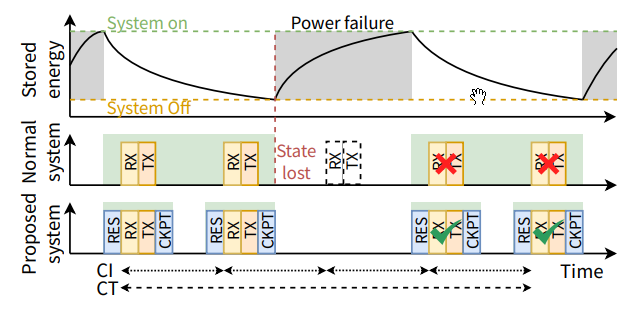
\includegraphics[width=0.8\textwidth,height=6cm,keepaspectratio=true]{images/intermittent_device_operation.png}
    \caption{
       Intermittently-powered device operation versus a conventionally-powered device operation (Figure taken from \cite{freebie}). When the conventional, non-protected system exhibits a power failure, all network state is lost, and the handshake procedure has to be fully restarted. An intermittently-powered device powers itself down in between network events in order to conserve energy as well as being able to fully recover from a power failure as if it was operating normally.
    }
    \label{fig:intermittent_operation}
\end{figure}

To conserve energy as much as possible, these devices often only power up parts of the system that are strictly necessary. This can take the form of the system only receiving power from its harvesting when being used (e.g., energy-harvesting buttons in smart light switches) or the system scheduling its own power-on events using low-power circuitry. This mode of operation is often called \textit{intermittent computing} and these devices \textit{intermittent} or \textit{intermittently-powered devices}. Figure \ref{fig:intermittent_operation} shows how these devices operate versus conventionally-powered devices.

Intermittently-powered operation makes wireless communication difficult. In the state-of-the-art solutions for intermittently-powered devices, Uni-directional communication has been achieved by advertising data when enough power is available. For example, bi-directional communication has been realized at a short range using RFID. With RFID technology, a reader ``interrogates'' a device that communicates back utilizing the principle of backscatter \cite{wisp_2005}. Although RFID is bi-directional, it requires a reader to energize the sensor devices at a short distance. As a result, medium-range, high throughput, intermittently-powered communication with active radios has not been possible until very recently. The system proposed by \cite{freebie}, called FreeBie, aims to solve this. It does so by using Bluetooth Low-energy and noting that, between transmission events, the System on Chip (SoC) could be powered down fully, only leaving on an ultra-low-power real-time clock (RTC) tasked with turning the SoC back on just in time for the next transmission. By doing so \cite{freebie} achieved the first ever battery-free devices capable of maintaining a wireless connection of a widely accepted standard. Even though BLE, as the name would suggest, has been developed for low-energy peripherals, its use within an intermittently-powered device has exposed some inefficiencies previously considered acceptable.

The work within this thesis will be based on the FreeBie system. By modifying the BLE stack source code, we aim to mitigate the inefficiencies of FreeBie. What these inefficiencies are will be discussed in the next section.

\section*{Problem Statement}
\label{sec:introduction_problem_statement}

To provide context, we would like to reiterate that intermittent devices receive power by harvesting ambient energy. Although the variability and unreliability of power is the root issue with energy harvesting systems, this can not be solved. However, it does provide context as to why the following issues do not exists with conventionally-powered BLE devices.

The first problem arises when the connection is formed. When the \textit{central}, for example, an Android phone, initiates a connection with a \textit{peripheral}, in this case FreeBie, it gets to decide the initial connection settings. These connection settings define the baseline connection speed and, as a result, the power consumption of the peripheral. After the connection setup, the peripheral can request more suitable connection parameters. However, this means that during the connection setup, we have to contend with the default connection parameters of the central. In the case of a phone running the Android operating system (OS), these settings are high-throughput and high power consumption. 

These unfavorable connection parameters forced FreeBie's designers to use capacitor sizes within FreeBie that, after the connection setup is finished, go mostly unused \cite{freebie}. This means the device as a whole increased in size and cost. 

The connection setup itself also has room for improvement. In the naive approach used in common frameworks, like Packetcraft and Zephyr, the connection setup is long and repetitive. For even a simple application, the number of packets required to set up can easily exceed 70 packets, which can be seen in Figure \ref{fig:static_packet_division}. At Android's fast settings, this already takes a few seconds. Using slower settings, which are more favorable for these ultra-low power devices, the setup can take up to three minutes. With more complex applications, these numbers increase rapidly.

Considering the variability of the power harvesting methods that these devices employ, it is often advantageous to switch to a faster connection configuration when plenty of energy is available or even crucial to switch to a slower connection configuration to protect against a power failure. Using the procedures available within the BLE specification, it takes a fixed six packets for the central to apply the connection settings after accepting them from the peripheral. This takes anywhere between tens of milliseconds to a minute, depending on the active connection parameters. 

Take as an example an intermittent device that takes its power from solar. If someone were to accidentally block the solar panel, then at the lowest connection settings, the device would not be able to throttle the connection fast enough to protect itself against a power failure. From all these remarks, we can gather at least three possible goals to improve BLE for use within intermittently-powered devices:
\begin{enumerate}
    \item \textbf{Goal 1}: Allow the Peripheral to dictate the initial connection parameters.
    \item \textbf{Goal 2}: Reduce the time required for the connection setup.
    \item \textbf{Goal 3}: Reduce the time required to apply new connection parameters.
\end{enumerate}
This thesis will address these the above three points with the general goal of improving the viability of BLE for intermittently-powered devices.

Chapter \ref{chp:chapter_2} covers the necessary background information. Chapter \ref{chp:chapter_3} will explain the architecture of the proposed solutions. Chapter \ref{chp:chapter_4} validates and evaluates the efficacy of these solutions. Chapter \ref{chp:futurework} will discuss future work. Finally, Chapter \ref{chp:conclusions} will draw a conclusion from the evaluation.


% Create chapters
\chapter{Background}
\label{chp:chapter_2}

In this chapter the necessary background information will be covered to be able to fully understand the architecture of the proposed solutions, as well as defining useful terms. 

\section{Wireless Connection}
\label{sec:ch2_wireless_connection}
A wireless connection is setup between at least two devices. Within the bluetooth low-energy specification there exists a clear hierarchy, where one device is dominent and is called the Central. The central usually takes the shape of a phone or a laptop. The other side of the connection is with one or more Peripherals. These devices include headphones, smartwatches, IoT sensors, pushbuttons and much more. 

For the sake of this thesis I define three phases for a BLE connection. These phases are:
\begin{itemize}
    \item \textit{Unconnected}: before any connection is established between the Central and the Peripheral
    \item \textit{Connection Setup}: starts from the connection request and ends when the last non-application packet is sent. 
    \item \textit{Application}: starts when connection setup is finished and only application packets are sent. Application packets are packets that are necessary to fullfil the application. 
\end{itemize}
These terms are not officially defined by the BLE specification, but are used throughout this thesis. 

\section{Advertisers and Scanners}
When in an unconnected state, the Peripheral and Central can take on the roles of \textit{Advertiser} and \textit{Scanner} respectively. As an Advertiser, a Peripheral sends out advertising packets. Advertising packets can contain up to 31 bytes of advertising data. The structure of the advertising data is shown in Figure \ref{fig:advdata_layout}. The \texttt{AD Type} field is an 8 bit identifier which refers to one of the many predefined advertisement datatypes. This is followed by the length of the data for this type and then the actual data. 

\begin{figure}[]
    \centering
    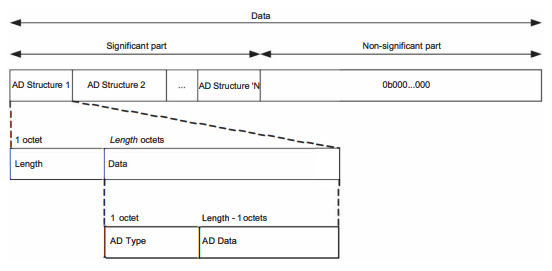
\includegraphics[width=0.8\textwidth,height=6cm,keepaspectratio=true]{images/advertising_data}
    \caption{
        The layout of the AdvData field for advertisement packets. Advertisement packets allow for 31 bytes of consecutive AD Structures. These structures contain the length of the structure, followed by the AD Type, and finally the AD Data as defined in the specification for that AD Type \cite{bluetooth_spec}.
    }
    \label{fig:advdata_layout}
\end{figure}

There are multiple different advertising modes, but the only one used in this thesis is the \texttt{ADV\_IND}. This mode has two traits which are \textbf{Connectable} and \textbf{Scannable}. Connectable means that the Peripheral is open for connection requests. Scannable means that a Central can, as a response to an advertising packet, send a \textit{Scan Request} to request more data from the Perihperal. This data is then sent in the form of a \textit{Scan Response} and allows for another 31 bytes of advertising data.

\section{Connection Parameters}
The connection setup is initiated by the Central by responding with a \texttt{CONNECT\_IND} packet to an advertisement packet. From this moment a connection between the devices is made and the setup can begin. The parameters which decide the connection configuration are contained within the \texttt{CONNECT\_IND} packet (\texttt{LLData} field). The most important configuration values to understand are \textit{Connection Interval} (CI) and \textit{Peripheral Latency} (PL). 

\begin{figure}[]
    \centering
    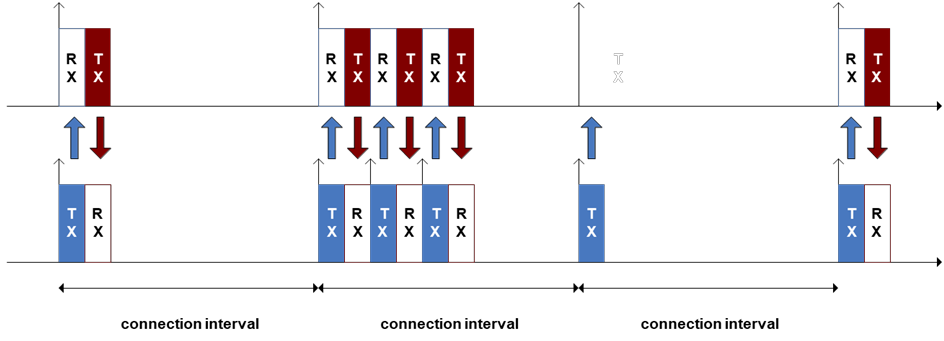
\includegraphics[width=0.8\textwidth,height=6cm,keepaspectratio=true]{images/connection_interval_slave_latency}
    \caption{
        An example timeline of communications between a \color{red} Peripheral \color{black} and \color{blue} Central \color{black}. At every connection interval a new chain of transmission events can start. This chain can theoretically continue up until the end of the connection interval. If the Perpipheral Latency is set to $N$, it allows the Peripheral to skip responding to $N$ connection interval events from the Central in order to conserve energy. This can be seen in the third spike \cite{nordic_2022}.
    }
    \label{fig:ci_and_pl}
\end{figure}

As you can see in Figure \ref{fig:ci_and_pl}, the Connection Interval is the time between the start of chains of transmit (TX) and receive (RX) events. Multiple TX/RX events can happen within one chain, but when there is no more data to be sent then the current chain is over and new data can be transmitted at the following interval. Peripheral Latency defines how many Connection Intervals the Peripheral is allowed to skip. For example, take a CI of 2 seconds and a PL of 0, this means that every two seconds the Central transmits a packet and the Peripheral replies. Now take a CI of 2 and a PL of 1, in this case the Central transmits every two seconds, but the Peripheral is allowed to sleep every other packet, effectively making the time inbetween transmissions four seconds. 


\begin{table}
    \begin{center}
    \begin{tabular}{|l|l|}
        \hline
        \textbf{Parameter} & \textbf{Constraints} \\
        \hline
        Connection Interval & Range: 0x0006 0x0C80 \\
                            & $Time = N * 1.25ms$ \\
                            & Time Range: 7.5ms to 4000ms \\
        \hline
        Peripheral Latency  & Range: 0x0000 to 0x01F3 \\
        \hline
        Supervision Timeout & Range: 0x000A to 0x0C80 \\
                            & $Time = N * 10ms$ \\
                            & Time Range: 100ms to 32s \\
                            & $Timeout \leq (Latency + 1) * Interval$ \\
        \hline
    \end{tabular}
    \end{center}
    \caption{Connection parameters and parameter constraints.}
    \label{tbl:conn_params}
\end{table}

The units and ranges for the three connection parameters are defined in Table \ref{tbl:conn_params}.

\section{Services and Characteristics}
\begin{figure}[]
    \centering
    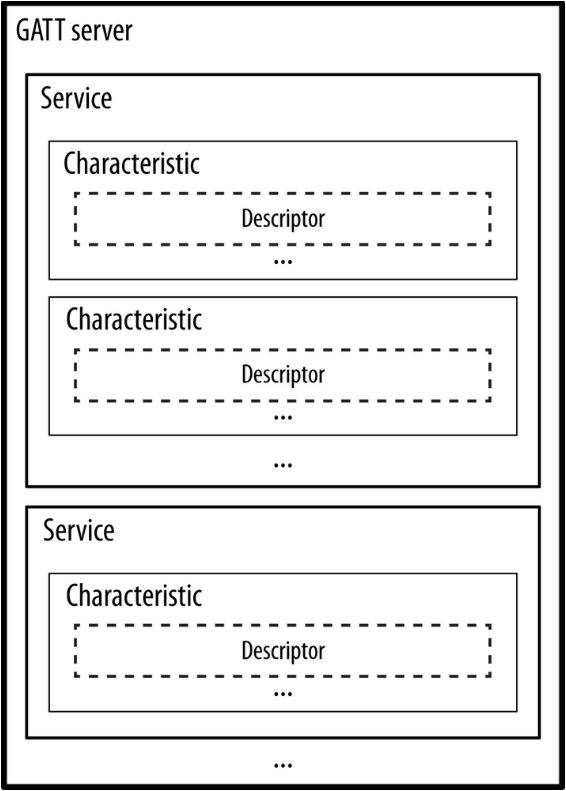
\includegraphics[width=0.5\textwidth,height=6cm,keepaspectratio=true]{images/gatt_service}
    \caption{
        The architecture of the GATT Server. Functionality is grouped as services. Services contain data as characteristics that can be read from or written to. Descriptors are used as metadata that describe each characteristics and for configuring the server to notify the client of updates from the characteristic they're grouped under \cite{townsend_cufi}.
    }
    \label{fig:gatt_server}
\end{figure}
The \textit{Generic Attribute Profile} (GATT) defines how profile and user data is exchanged over a BLE connection. GATT defines the GATT Server, within which functionality is split up into \textit{Services}. Services contain datapoints called \textit{Characteristics}. These characteristics can be interpreted and configured using fields called \textit{Descriptors}. See Figure \ref{fig:gatt_server} for a schematic layout of the GATT Server.

\begin{figure}[]
    \centering
    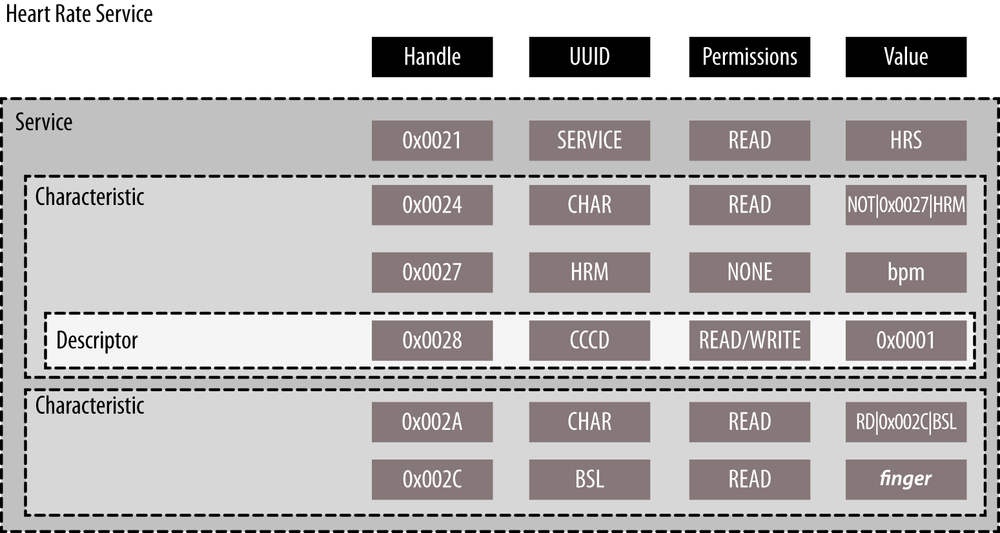
\includegraphics[width=0.5\textwidth,height=6cm,keepaspectratio=true]{images/heartrate_service}
    \caption{
        An example of a service. Each element is searchable through its UUID and then uniquely identifiable using its consecutively numbered handle \cite{townsend_cufi}.
    }
    \label{fig:hrs_layout}
\end{figure}
To give a real world example, take the Heart Rate Service in Figure \ref{fig:hrs_layout}. This service allows a Client to read the heartrate sensor of a device. The heartrate service contains a characteristic called Heartrate. One of the descriptors tells us that the unit is defined as \textbf{beats per minute}. We could read the characteristic value manually, but if we would like to be notified when a new measurement is done then we can set the Notify bit of the \textit{Client Characteristic Configuration} or CCC descriptor.

To be able to read or write to a Characteristic we need its handle. The handle is a number that is unique for a characteristic within a GATT Server. To find this handle we can perform a \textit{Find By Type Request} using its 16-bit Universally Unique Identifier (UUID). Bluetooth SIG has predefined UUIDs for many predefined Services. Each predefined Service has a specification which defines the shape of the service. This includes all the Characteristics, Descriptors and their respective UUIDs.

The process of finding all these handles is what is called \textit{Service Discovery}. The result of this process is a list of numbers that can be used to read and write to the server. After Service Discovery is done the GATT Servers need to be configured. This usually means writing to the CCC descriptor to setup notifications for the desired Characteristics. This process will henceforth be refered to as Configuration. 

Both the Central and the Peripheral can be Servers and Clients at the same time. For example; a phone can provide the central time for a smartwatch to display on the watchface, while the smartwatch measures the heartrate for the phone to display within a health application. This means that a Service Discovery and Configuration needs to be performed by both the Central and the Peripheral.

\section{Link Layer}
The Link Layer is the part of the Bluetooth stack which is tasked with managing the wireless link and actually sending data frames. The Link Layer sits inbetween the higher level protocols like GAP and GATT and the Physical Layer which actually controls the radio.
Procedures are defined within the Link Layer to make sure both the transmitting radio and receiving are configured correctly.

The \textit{Features Exchange} procedure is used to exchange which features are supported by both radios. These feature sets can vary widely between versions of Bluetooth and can have a large impact on performance. To guarantee that both sides of the link communicate in the same manner, these features are exchanged by the Link Layer at the start of each connection.

The size of the packets that can be received by a radio can also vary and is usually dependent on the available memory. To make sure the best throughput is achieved this needs to be communicated using the \textit{Data Length Exchange}. This exchanges the largest Air packet that each radio is able to receive at once.

\section{Connection Setup}
As previously defined in Section \ref{sec:ch2_wireless_connection}, the connection setup starts from the Connection Request and ends when the last non-application packet is sent. The packets that occur during Connection Setup can be divided into four groups which correspond to the subjects discussed in the previous sections.
\begin{itemize}
    \item Link Layer
    \item Service Discovery
    \item Configuration
    \item Application
\end{itemize} 
The order in which they occur are usually Service Discover, Configuration and then Application, with Link Layer communication starting parallel to the Service Discovery from the start.

\section{Operating Systems}
The FreeBie project was originally developed using the open-source BLE stack Packetcraft. Due to its architecture it was especially suitable to be modified in the way required for intermittent operation. This is because all OS tasks are managed using a single scheduler which uses a generic sleep method. This sleep method was altered to configure the real-time clock (RTC), dump the memory to FRAM, and to fully power down the SoC.

However, since FreeBie was originally developed, Packetcraft has gone into closed-source development. For this reason, a newer RTOS was chosen for the Central. Zephyr OS is a modern RTOS developed by the Linux Foundation and is now the officially supported stack for Nordic Semiconductors.

**something extra about modifying link layer stack
\chapter{Connection Setup and Parameter Adaption}
\label{chp:chapter_3}

This chapter describes the ... In Section~\ref{sec:SECTIONTITLE}, examples are given om how to use tables and figures in this MSc thesis.

\section{SECTION TITLE}
\label{sec:SECTIONTITLE}

\chapter{Evaluation}
\label{chp:chapter_4}
The evaluation of our system is split up in a \textit{static} and a \textit{dynamic} part. The static evaluation quantifies the connection setup performance for each optimization stage. The static behavior will be benchmarked on \textit{number of packets during connection setup}, \textit{connection setup time}, \textit{connection parameter update time}, \textit{time until first useful packet}, and \textit{power consumption}. The dynamic evaluation is about quantifying the performance of FRAPPUCcInO, which will be based on \textit{average throughput}, and \textit{responsiveness}.

This separation is made because the static performance improvement will be applicable to both intermittently-powered and conventionally-powered devices. Reducing connection setup time and power consumption on their own are attractive propositions since it improves responsiveness and battery life. The FRAPPUCcInO algorithm is not the only possible application of \textit{Fast Reconnect}. For example, Fast Reconnect could also be leveraged to quickly build a connection when ambient energy is insufficient for even the maximum connection interval, allowing a pseudo-connected state. 

% \section{Experimental Setup}
\label{sec:evaluation_setup}
The demo system described in Section \ref{sec:demo_application} was also used in all experiments. The central is an nRF52840DK development board \cite{nordic_nrf52840dk}, and the peripheral is the modified FreeBie platform \cite{freebie}. The nRF52840-Dongle was used as a sniffer for Wireshark \cite{nordic_dongle}. During the static testing, the Nordic Power Profiler Kit II (PPK-II, \cite{nordic_ppk2}) was used to power FreeBie and measure its power consumption. During the dynamic testing, the PPK-II was replaced with a 46.5$\mu\text{W}$ solar cell from Panasonic \cite{panasonic_solar}, and a Saleae Logic Pro 8 was used to capture digital and analog traces \cite{saleae_logic_pro_8}. Finally, an Ikea TRÅDFRI smart light was calibrated and controlled through \texttt{python} to simulate changing energy harvesting conditions. 

The \texttt{CMakeLists} file of both applications have been retrofitted to enable easy switching between optimization stages during testing. To enable a specific stage, the \texttt{CMake} variables must be set according to Table \ref{tbl:stage_defs}.
\begin{table}
    \begin{center}
    \begin{tabular}{|l|l|l|l|l|}
        \hline
                                & \multicolumn{4}{c|}{\textbf{Stage}}   \\
        \textbf{Variable}    & \textbf{1} & \textbf{2} & \textbf{3} & \textbf{4} \\
        \hline
        CACHE\_SERVICE\_DISCOVERY &   & 1 & 1 & 1 \\
        \hline
        SKIP\_RECONF             &   &   & 1 & 1 \\
        \hline
        CACHE\_LL\_FEAT\_EXCH      &   &   &   & 1 \\
        \hline
        CACHE\_LL\_DL\_EXCH        &   &   &   & 1 \\
        \hline
    \end{tabular}
    \end{center}
    \caption{\texttt{CMake} variables to set for a given optimization stage. Set the variable to 1 if the cell contains a 1, otherwise do not set the variable.}
    \label{tbl:stage_defs}
\end{table}

\section{Results}
\label{sec:evaluation_results}

\subsection{Static Evaluation}
\label{sec:static_evaluation}
% Number of Packets Plot
\begin{figure}[]
    \centering
    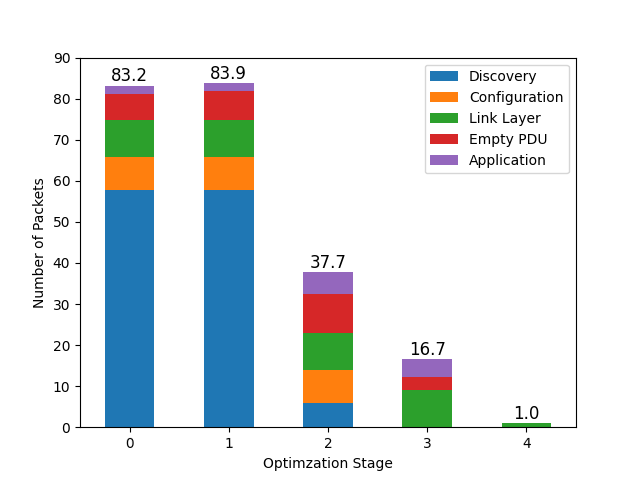
\includegraphics[width=0.5\textwidth,height=6cm,keepaspectratio=true]{plots/static_packet_division.png}
    \caption{
        Number of packets from the \texttt{CONNECT\_IND} up to the last connection setup packet.
    }
    \label{fig:static_packet_division}
\end{figure}

Between the number of packets sent between the \texttt{CONNECT\_IND} packet and the first packet that does not belong to the connection setup, shown in Figure \ref{fig:static_packet_division}, a significant reduction can be seen. From Stage 0 (no modifications) to Stage 4 (all modifications) this is a reduction of \textbf{98.80\%}. When only sharing the preferred (slower) connection parameters (Stage 1), the average number of packets goes up by 0.7 packets. This increase in packets is a result of slightly more Empty PDUs as a result of different timing. Stage 2 still counts six packets for \textit{discovery}, even though service discovery caching is being used because reading the Database Hash requires three packets for both the central and peripheral. 

% Setup Time Plot
\begin{figure}[]
    \centering
    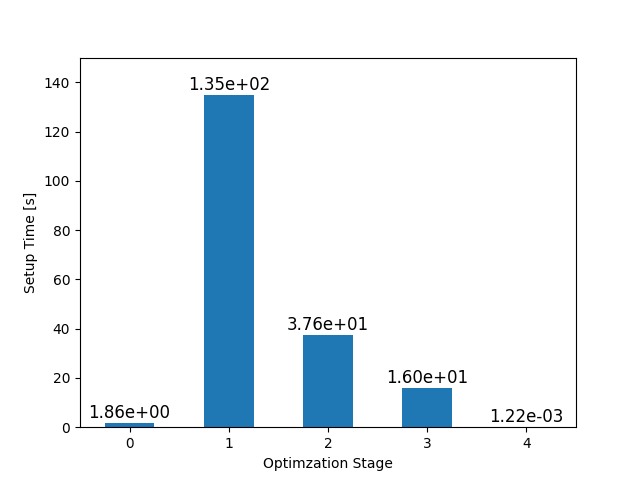
\includegraphics[width=0.5\textwidth,height=6cm,keepaspectratio=true]{plots/static_setup_time.png}
    \caption{
        Connection setup time, measured from \texttt{CONNECT\_IND} up to the last packet that does not belong to the connection setup.
    }
    \label{fig:static_setup_time}
\end{figure}

Figure \ref{fig:static_setup_time} shows the time required to set up a connection, measured from \texttt{CONNECT\_IND} up to the last packet that does not belong to the connection. At first, Stage 1 through 3 seems significantly worse than stage 0. However, it is important to remember that in Stage 0, the peripheral is forced to use the default connection parameters of the central. As a result, our system needs to be designed with a much larger capacitor than required after the connection is established. Although slower, Stage 1 allows us to reduce the size of the capacitors used in our system, which allows the system to recover much faster after a full power failure, as well as reducing the overall size and cost of the system. Stage 4 reduces the connection setup to a single packet, resulting in a reduction of \textbf{99.93\%} compared to Stage 0.

% Time To Useful Packet Plot
\begin{figure}[]
    \centering
    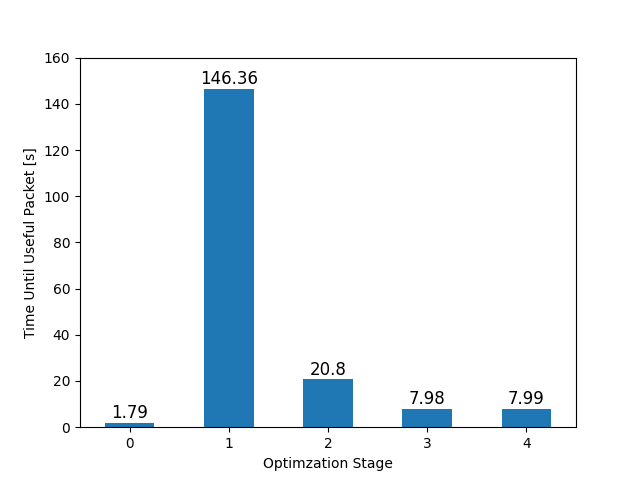
\includegraphics[width=0.5\textwidth,height=6cm,keepaspectratio=true]{plots/static_useful_packet_time.png}
    \caption{
        Time until the first useful packet. Measured from \texttt{CONNECT\_IND} up to the first useful application packet.
    }
    \label{fig:static_useful_packet_time}
\end{figure}

To measure the fastest possible time until a useful packet is received by the central, we perform a \textit{Read Request} from the central on the \textit{battery level} characteristic. A \textit{useful packet} is defined as anything that directly contributes to the function of an application. For example, a read or write request on a characteristic, or a write request on a CCC to enable Notifications. 

From Figure \ref{fig:static_useful_packet_time} one can see that Stage 4 is about 4.46 times slower than Stage 0. However, the default connection interval used by Zephyr in Stage 0 is 50 milliseconds, which is 80 times slower than the connection interval used by Stage 4. The improvements in Stages 2, 3, and 4 are able to recoup a significant amount of the time gained by using the slowest connection parameters, which is visible from Stage 1 in Figure \ref{fig:static_useful_packet_time}. It is also notable that eight seconds is the lower limit that is possible at a connection interval of four seconds since a complete read operation from a GATT server requires two packets. The fact that there is no decrease from Stage 3 to Stage 4 is supported by the idea that the link layer procedures 

% Connection Adaption Time vs. current CI
\begin{figure}[]
    \centering
    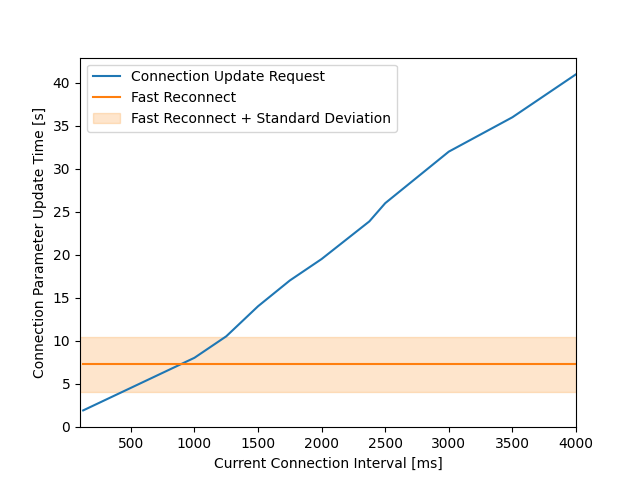
\includegraphics[width=0.5\textwidth,height=6cm,keepaspectratio=true]{plots/static_conn_update_plot.png}
    \caption{
        Time until new connection parameters are applied versus currently used connection parameters.
    }
    \label{fig:static_conn_update_time}
\end{figure}

Figure \ref{fig:static_conn_update_time} shows the time it takes for new connection parameters to be applied when using the regular \textit{connection update request} versus \textit{Fast Reconnect}. Since the time required to reconnect using fast reconnect is independent of the connection interval, the time to update connection parameters does not increase as the connection interval increases. However, fast reconnect is more variable since it requires the central to receive a new advertisement from the peripheral. One standard deviation is shown in Figure \ref{fig:static_conn_update_time} with light orange. An optimal approach would use the conventional connection update request when CI is below 1250, and fast reconnect for CI above 1250.

% Energy Used vs. Optimzation Stage
\begin{figure}[]
    \centering
    \begin{minipage}[b]{0.47\textwidth}
      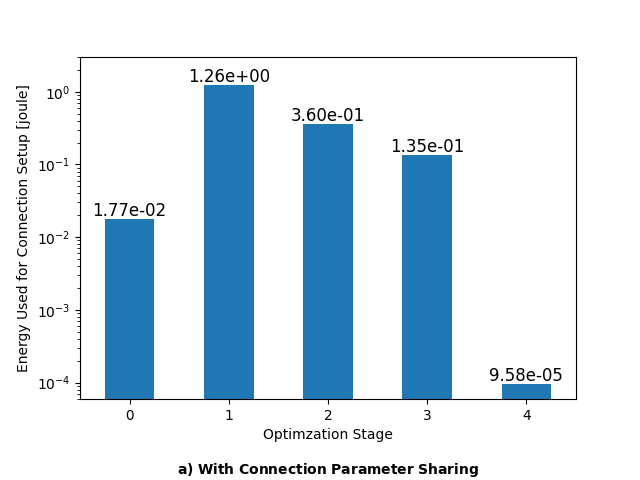
\includegraphics[width=\textwidth]{plots/static_power_consumption_conventional.png}
    \end{minipage}
    \hfill
    \begin{minipage}[b]{0.47\textwidth}
        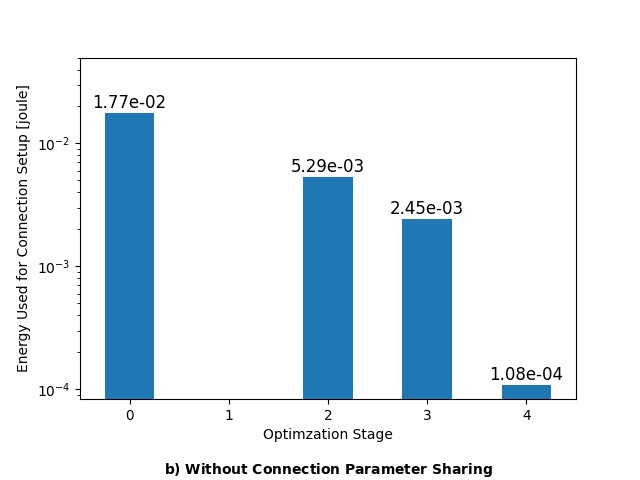
\includegraphics[width=\textwidth]{plots/static_power_consumption_conventional_fast.png}
    \end{minipage}
    \caption{Energy consumed (in Joule) during connection setup versus optimization stage when conventionally-powered. a) Uses Connection Parameter Sharing (Stage 1). b) Does not use Connection Parameter Sharing.}
    \label{fig:static_power_consumption_conventional}
\end{figure}

As one can see in Figure \ref{fig:static_power_consumption_conventional}a, when conventionally powered and using slow connection parameters, the total energy consumed only drops below Stage 0 when using all optimizations. This is because the microcontroller is still using power while idling, so extending the setup time by increasing the connection interval will cause higher energy usage. However, when using all optimizations, the energy usage is \textbf{reduced by 99.46\%}. When using these optimizations in devices that do not employ energy harvesting, it is advised to reduce the connection parameters after the setup process is done. This is shown in Figure \ref{fig:static_power_consumption_conventional}b.

\begin{figure}[]
    \centering
    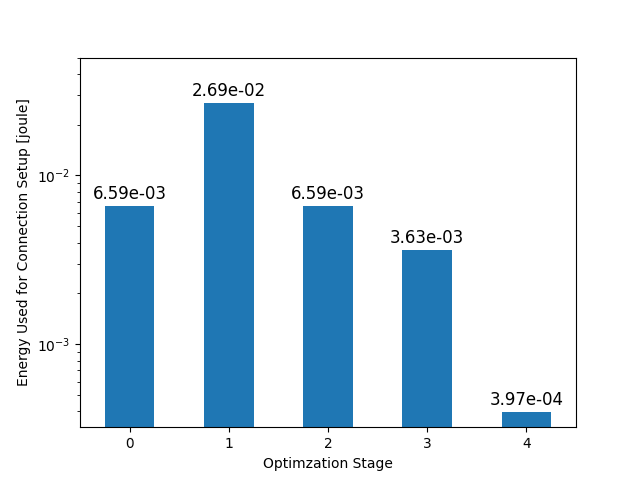
\includegraphics[width=0.5\textwidth,height=6cm,keepaspectratio=true]{plots/static_power_consumption_intermittent.png}
    \caption{
        Energy consumed (in Joule) during connection setup versus optimization stage when intermittently-powered. 
    }
    \label{fig:static_power_consumption_intermittent}
\end{figure}

Figure \ref{fig:static_power_consumption_intermittent} shows the energy used during the connection setup while intermittently-powered. Stage 3 and 4 show a significant reduction in energy consumed with \textbf{44.96\%} and \textbf{93.97\%}, respectively. However, Stage 1 and 2 might still be an improvement when intermittently-powered since the average current draw during connection setup is 68.96$\mu$A, and 71.13$\mu$A, compared to 1.21mA of Stage 0. This reduced continuous current draw might allow an intermittently-powered device to remain operational using Stage 1, while Stage 0 would result in the capacitor voltage becoming critically low.

\subsection{Dynamic Evaluation}
\label{sec:dynamic_evaluation}
\begin{figure}[]
    \centering
    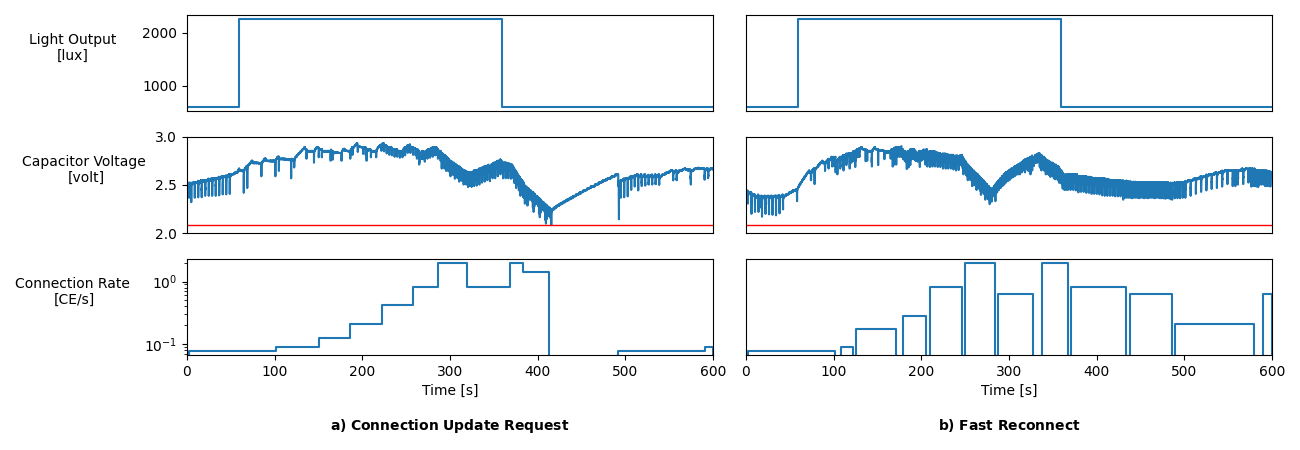
\includegraphics[width=0.96\textwidth,keepaspectratio=true]{plots/dynamic_short_both.png}
    \caption{
        Connection Rate versus Light Output. The average throughput when using Fast Reconnect (b) is 24.29\% higher and the peak throughput comes 15.86\% earlier when compared to using the regular Connection Update Request (a).
    }
    \label{fig:dynamic_short_both}
\end{figure}

Figure \ref{fig:dynamic_long_both} shows an optimal situation for using FRAPPUCcIno, which is a sharp increase followed by a sharp decrease in available power after using slow connection parameters. In this scenario, using Fast Reconnect allows an earlier rise, as well as allowing the system to respond in time to prevent a power failure. As a result, FRAPPUCcInO using Fast Reconnect is able to maintain an average throughput of \textbf{24.29\%} higher when compared to FRAPPUCcInO using the regular Connection Update Request. We define the responsiveness as the peak-to-peak time between the \textit{light output} and the \textit{connection rate}. Using this definition, FRAPPUCcInO with Fast reconnect reaches its peak 191 seconds after the light output rises, and FRAPPUCcInO using Connection Update Request reaches its peak after 227 seconds. The responsiveness is therefore improved by \textbf{15.86\%}.


\begin{figure}[]
    \centering
    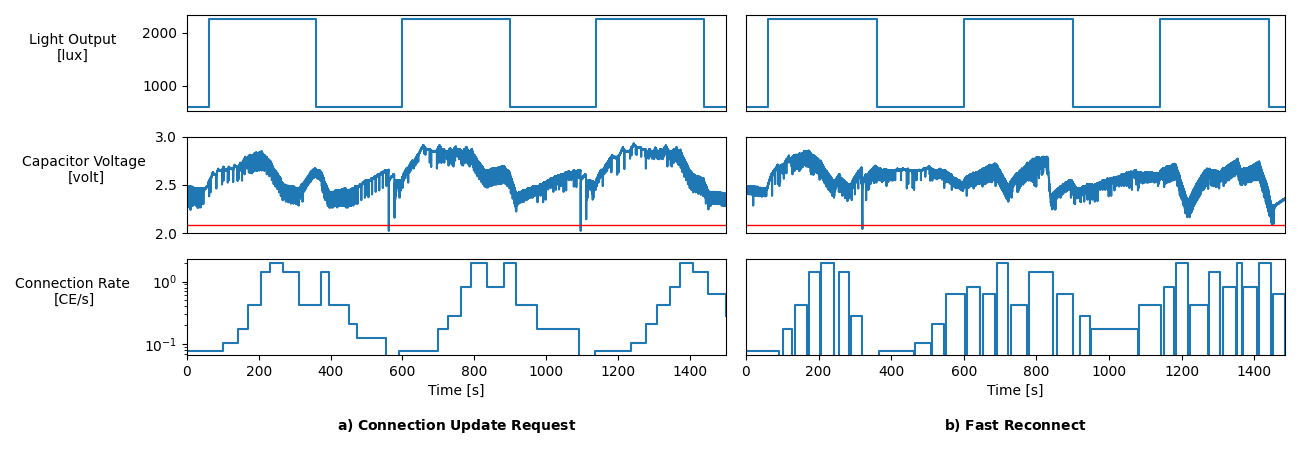
\includegraphics[width=0.96\textwidth,height=6cm,keepaspectratio=true]{plots/dynamic_long_both.png}
    \caption{
        Connection Rate versus Light Output. \textbf{left}) Connection Update Request. \textbf{right}) Fast Reconnect.
    }
    \label{fig:dynamic_long_both}
\end{figure}

When performing a long run, the advantage in throughput is less drastic but still significant. Figure \ref{fig:dynamic_long_both} shows a 25 minute run with multiple peaks in light output. In this scenario, the average throughput is \textbf{10.87\%} higher for FRAPPUCcInO using Fast Reconnect. However, responsiveness has improved by \textbf{107\%}. This improvement can be attributed to the fact that FRAPPUCcInO with Fast Reconnect is able to decrease the throughput earlier to start charging the capacitor up. As a result, FRAPPUCcInO reaches the voltage where it can increase the throughput again much earlier. We should note that during runs longer than 15 minutes, both systems were very like to encounter hard faults. These instability issues should be fixed before we are able to fully assess the performance of FRAPPUCcInO over longer periods.

% Create conclusions
\chapter{Conclusions}
\label{chp:conclusions}

We have presented a new method of reducing connection setup overhead and energy usage in Bluetooth Low-Energy (BLE) for battery-less devices, as well as conventional battery-powered devices. This method is called Fast Reconnect and is platform agnostic. Fast Reconnect applies caching in multiple levels of the BLE stack, from the GATT layer all the way down to the link layer, to reduce the connection setup process to a single packet. To improve connection parameter adaption time within FreeBie, we also presented FRAPPUCcInO, which combines Fast Reconnect with a control system to improve throughput and responsiveness under highly variable energy harvesting conditions. Using Fast Reconnect, together with FRAPPUCcInO, intermittent devices can become smaller, perform with even less ambiently available energy, and even enjoy a more responsive user experience.

% Create future work
\chapter{Future Work}
\label{chp:futurework}

While the method of sharing connection parameters within the advertisement data works, it requires compliance from the central to work. Further research could focus on standardising the procedures around sharing the connection parameters, so that other platforms can support this feature and Bluetooth Low-Energy becomes more hospitable to batteryless devices.

Although Fast Reconnect covers all link layer communication used by our demo application, further testing needs to be done to assess of our method can be applied to all link layer exchanges. A generic approach, built into the link layer controller, would be ideal and would guarantee support for future revisions of BLE.

Finally, while FRAPPUCcInO provides some promising initial results, it is clear that furthur work is required to improve stability, and to optimize the algorithm further. A combination between using \textit{Fast Reconnect} and the regular \textit{connection parameter update request} as the methods of applying parameters could prove even more effective.

% Create bibliography
\bibliographystyle{plain} % Please do not change the style of bibliography (yes, it should be `plain`)
\bibliography{./bib/MyMScTUDENSThesisBibFile}

% Create appendix
\appendix
\chapter{Demo System}
\label{app:appendix_a}
This appendix includes supplementary information on the features of the demo system, as well as a description of how it was implemented and developed.

\section{Using the System}
\subsection{Connecting and Powering the System}
\label{sec:connecting_setup}
Connecting and powering up the ``development'' configuration shown in Figure \ref{fig:demo_layout} is as simple as connecting both development boards to a computer using two micro USB to USB A cables. Be sure to check if all power switches are set to the ON position.

Connecting and powering the ``testing'' configuration shown in Figure \ref{fig:demo_layout} is a bit more involved. The central is connected to the computer using a micro USB-to-USB A cable like in the development setup. Connect FreeBie to a Segger JLink debug probe using a 5-pin debug cable. Attach the debug probe to the computer using a USB B-to-USB A. Power the FreeBie using the Nordic Power Profiler Kit II (PPK2), by connecting the the \textit{Vout} and \textit{Gnd} on the PPK2 to the \textit{Vbat} and \textit{Gnd} on FreeBie. Finally, download and open the Power Profiler application and change the settings to \textit{Volt Meter} and \textit{2660mV}.

\subsection{Using the Terminal}
\label{sec:using_terminal}
\begin{table}[H]
    \centering
    \begin{tabular}{|l|p{6cm}|}
    \hline
    \textbf{Command}  & \textbf{Help} \\
    \hline 
    \texttt{ble list show} & Show all discovered devices. \\ \hline
    \texttt{ble list find <local name>}  & Find device by name. \\ \hline
    \texttt{ble connect <index>} & Connect to a device using its index in the device list. \\ \hline
    \texttt{ble disconnect} & Terminate the current connection using the \textit{Remote User Terminated Connection} reason. \\ \hline
    \texttt{ble conn reconnect} & Terminate the current connection using the \textit{Fast Reconnect} reason. \\ \hline
    \texttt{ble cache delete <name>} & Delete the cached data and hash of an entry by name (e.g. "handles"). \\ \hline
    \texttt{ble cache scramble <name>} & Scramble the cached hash of an entry by name (e.g. "handles").  \\ \hline
    \texttt{ble cts notify} & Trigger a notification for the Current Time characteristic of the Central Time Service. \\ \hline
    \texttt{ble test read} & Perform a large read request ($\geq 27$ bytes) on the Test characteristic of the Test service. Used to validate \textit{LE Data Length Extension} caching. \\ \hline
    \texttt{ble test write} & Perform a large write request ($\geq 27$ bytes) on the Test characteristic of the Test service. Used to validate \textit{LE Data Length Extension} caching. \\ \hline
    \end{tabular}
    \caption{Terminal commands available on the central.}
    \label{tbl:demo_commands}
\end{table}

\begin{table}[H]
    \centering
    \begin{tabular}{|l|p{6cm}|}
    \hline
    \textbf{Command}  & \textbf{Help} \\
    \hline 
    \texttt{disconnect <id> [--fast]} & Terminate a connection by id (usually 1) using the \textit{Remote User Terminated Connection} reason (or \textit{Fast Reconnect} when the "--fast" flag is added). \\ \hline
    \texttt{param\_update <preset index>} & Perform a parameter update to a predefined preset using \textit{Fast Reconnect}. \\ \hline
    \end{tabular}
    \caption{Terminal commands available on the peripheral}
    \label{tbl:demo_commands_peripheral}
\end{table}
When the development boards are connected to the laptop, virtual COM ports are created on \texttt{/dev/ttyACM0}, \texttt{/dev/ttyACM1}, etc. A serial terminal application, such as \textit{PuTTY}, can be used to connect to the central and peripheral with a baud rate of 115200 bits per second. When connected, a \texttt{help} command can be entered to display the available commands.

Table \ref{tbl:demo_commands} and Table \ref{tbl:demo_commands_peripheral} show commands that can be invoked on the central and peripheral, respectively. These commands are used to perform basic functions required for testing new code and specific procedures to validate caching methods.

\subsection{Making a Connection}
To perform a connection setup, use the following steps:
\begin{enumerate}
    \item Connect and power on the central and peripheral as described in Section \ref{sec:connecting_setup}.
    \item Open a terminal session to the central using the method described in Section \ref{sec:using_terminal}.
    \item Enter \texttt{ble list show} and look for the local name ``Watch'' or enter \texttt{ble list find Watch} if the list exceeds the terminal size.
    \item Enter \texttt{ble connect <index>}, where \texttt{index} is the index of the device entry found in the previous step.
\end{enumerate}

\subsection{GATT Services and Characteristics}
\label{sec:app_a_services}

% Please add the following required packages to your document preamble:
% \usepackage{multirow}
\begin{table}[H]
    \centering
    \begin{tabular}{|l|l|l|l|}
    \hline
    \textbf{Service}      & \textbf{Characteristic}                    & \textbf{UUID} & \textbf{Perm.} \\ \hline
    \multirow{4}{*}{GAP}  & Device Name                                & 0x2A00        & R              \\ \cline{2-4} 
                          & Appearance                                 & 0x2A01        & R              \\ \cline{2-4} 
                          & Central Address Resolution                 & 0x2AA6        & R              \\ \cline{2-4} 
                          & PPCP                                       & 0x2AC9        & RW             \\ \hline
    \multirow{4}{*}{GATT} & Service Changed                            & 0x2A05        & R              \\ \cline{2-4} 
                          & Service Changed CCC                        &               & RW             \\ \cline{2-4} 
                          & Client Supported Features                  & 0x2B29        & RW             \\ \cline{2-4} 
                          & Database Hash                              & 0x2B2A        & R              \\ \hline
    \multirow{2}{*}{CTS}  & Current Time                               & 0x2A2B        & RWN            \\ \cline{2-4} 
                          & Current Time CCC                           &               & RW             \\ \hline
    \multirow{5}{*}{Test} & Supported New Alert Category               & 0x2A47        & R              \\ \cline{2-4} 
                          & New Alert                                  & 0x2A46        & N              \\ \cline{2-4} 
                          & Supported Unread Alert Category            & 0x2A48        & R              \\ \cline{2-4} 
                          & Unread Alert Status                        & 0x2A45        & N              \\ \cline{2-4} 
                          & Alert Notification Control Point           & 0x2A44        & W              \\ \hline
    \end{tabular}
    \caption{Services that are available in the central application. Permissions have been abbreviated in the permissions (perm.) column to R for Read, W for Write, and N for Notification}
    \label{tbl:services_central}
\end{table}

\begin{table}[H]
    \centering
    \begin{tabular}{|l|l|l|l|}
        \hline
    \textbf{Service}         & \textbf{Characteristic}         & \textbf{UUID} & \textbf{Perm.}  \\ \hline
    \multirow{4}{*}{GAP}     & Device Name                     & 0x2A00        & R               \\ \cline{2-4} 
                             & Appearance                      & 0x2A01        & R               \\ \cline{2-4} 
                             & Central Address Resolution      & 0x2AA6        & R               \\ \cline{2-4} 
                             & Resolvable Private Address Only & 0x2AC9        & R               \\ \hline
    \multirow{5}{*}{GATT}    & Service Changed                 & 0x2A05        & R               \\ \cline{2-4} 
                             & Service Changed CCC             &               & RW              \\ \cline{2-4} 
                             & Client Supported Features       & 0x2B29        & RW              \\ \cline{2-4} 
                             & Database Hash                   & 0x2B2A        & R               \\ \cline{2-4} 
                             & Server Supported Features       & 0x2B3A        & R               \\ \hline
    \multirow{2}{*}{Battery} & Battery Level                   & 0x2A19        & R               \\ \cline{2-4} 
                             & Battery Level CCC               &               & RW              \\ \hline
    \multirow{2}{*}{Test}    & Text                            &               & RW              \\ \cline{2-4} 
                             & Text CCC                        &               & RW              \\ \hline
    \end{tabular}
    \caption{Services that are available in the peripheral application. Permissions have been abbreviated in the permissions (perm.) column to R for Read, W for Write, and N for Notificatio}
    \label{tbl:services_peripheral}
\end{table}

Table \ref{tbl:services_central} and Table \ref{tbl:services_peripheral} show the services and characteristics that were added to the central and peripheral applications, respectively. If a specific use is mentioned in the table, then it was explicitly added to validate our modifications. The remaining services and characteristics provide a more realistic workload when testing service discovery.

\section{System Implementation}
\subsection{Packetcraft}
\subsubsection{Registering GATT Services with the ATT server}
In this example, it is shown how to add a simple GATT service with a single characteristic that contains the string ``Lorem ipsum''. First, define three variables for the service declaration, characteristic declaration, and the characteristic value.
\begin{lstlisting}
/* Test service declaration */
static const uint8_t testValSvc[] = {TEST_UUID_SERVICE};
static const uint16_t testLenSvc = sizeof(testValSvc);

/* Test text characteristic */
static const uint8_t testValTxtCh[] = {ATT_PROP_READ | ATT_PROP_WRITE, UINT16_TO_BYTES(TEST_TXT_HDL), TEST_UUID_TEXT};
static const uint16_t testLenTxtCh = sizeof(testValTxtCh);

/* Test text value */
static uint8_t testValTxt[TEST_TXT_LEN] = { 'L','o','r','e','m',' ','i','p','s','u','m', 0 };
static const uint16_t testLenTxt = sizeof(testValTxt);
\end{lstlisting} 
These variables can be used to describe the ATT attributes that make up the GATT service.
\begin{lstlisting}
static const attsAttr_t testList[] =
{
    /* Service declaration */
    {
        attPrimSvcUuid,
        (uint8_t *) testValSvc,
        (uint16_t *) &testLenSvc,
        sizeof(testValSvc),
        0,
        ATTS_PERMIT_READ
    },
    /* Characteristic declaration */
    {
        attChUuid,
        (uint8_t *) testValTxtCh,
        (uint16_t *) &testLenTxtCh,
        sizeof(testValTxtCh),
        0,
        ATTS_PERMIT_READ
    },
    /* Characteristic value */
    {
        testTxtUuid,
        testValTxt,
        (uint16_t *) &testLenTxt,
        sizeof(testValTxt),
        (ATTS_SET_UUID_128 
        | ATTS_SET_READ_CBACK 
        | ATTS_SET_WRITE_CBACK),
        (ATTS_PERMIT_READ | ATTS_PERMIT_WRITE)
    },
};
\end{lstlisting} 
Finally, the GATT service can be registered with the ATT server.
\begin{lstlisting}
/* Test group structure */
static attsGroup_t svcTestGroup =
    {
        NULL,
        (attsAttr_t *) testList,
        NULL,
        NULL,
        TEST_START_HDL,
        TEST_END_HDL
    };
    
AttsAddGroup(&svcTestGroup);
\end{lstlisting}

\subsubsection{Supporting Notifications for a Client}
To allow a GATT client to enable Notifications on a characteristic using its CCC descriptor, we need to register the CCCs with the ATT server. To do this we first define the CCC set.
\begin{lstlisting}
/*! enumeration of client characteristic configuration descriptors */
enum
{
    APP_BATT_LVL_CCC_IDX,  /*! Battery Level */
    APP_CCC_COUNT
};

/*! client characteristic configuration descriptors settings, indexed by above enumeration */
static const attsCccSet_t appCccSet[APP_NUM_CCC_IDX] =
{
    /* APP_BATT_LVL_CCC_IDX */
    {
        BATT_LVL_CH_CCC_HDL,   // ccc handle
        ATT_CLIENT_CFG_NOTIFY, // value range
        DM_SEC_LEVEL_NONE      // required security level
    }   
};
\end{lstlisting}
The CCC set can then be registered with the ATT server.
\begin{lstlisting}
static void appCccCback(attsCccEvt_t *pEvt)
{
    /* Perform any necessary action to enable or disable notifications, like starting periodic timers. */
}

AttsCccRegister(APP_CCC_COUNT, (attsCccSet_t *) appCccSet, appCccCback);
\end{lstlisting}

\subsubsection{Service Discovery}
To discover a single service, define a list of characteristics to discover. Afterward, perform a service discovery using the characteristic list and pass the function a pointer to the global handle list.
\begin{lstlisting}
uint16_t globalHandleList[2] = {};

/* Characteristic 1 */
static const attcDiscChar_t ch1 =
{
    Characteristic1Uuid, /* uuid */
    ATTC_SET_UUID_128 /* optional characteristic settings */
};

/* Characteristic 1 */
static const attcDiscChar_t ch2 =
{
    Characteristic2Uuid,
    0
};

/*! List of characteristics to be discovered; order matches handle index enumeration  */
static const attcDiscChar_t *charList[] =
{
    &ch1,
    &ch2
};

AppDiscFindService(connId, 
                    ATT_16_UUID_LEN, 
                    (uint8_t *) ServiceUuid,
                    GATT_HDL_LIST_LEN, 
                    (attcDiscChar_t **) charList, 
                    globalHandleList);
\end{lstlisting}

\subsubsection{Configuration of a Remote GATT Server}
Configuration consists of initial reads from and writes to characteristics and enabling notifications for characteristics. However, since notifications are enabled by writing to the CCC descriptor of a characteristic, configuration is essentially only initial reads from and writes to characteristics. Packetcraft automates configuration by allowing us to define a list of characteristics to read from or write to automatically. For example, first define a list containing an initial read on the Central Time characteristic, as well as writing to the Central Time CCC descriptor to get updates of the Central Time in the future.
\begin{lstlisting}
/* Default value for CCC notifications */
static const uint8_t watchCccNtfVal[] = {UINT16_TO_BYTES(ATT_CLIENT_CFG_NOTIFY)};

/* List of characteristics to configure after service discovery */
static const attcDiscCfg_t discoveryConfig[] =
{
  /* Read:  CTS Current time */
  {NULL, 0, (TIPC_CTS_CT_HDL_IDX + WATCH_DISC_CTS_START)},

  /* Write:  CTS Current time ccc descriptor */
  {watchCccNtfVal, sizeof(watchCccNtfVal), (TIPC_CTS_CT_CCC_HDL_IDX + WATCH_DISC_CTS_START)},
};

AppDiscConfigure(connId, 
                APP_DISC_CFG_START, 
                WATCH_DISC_SLAVE_CFG_LIST_LEN,
                (attcDiscCfg_t *) discoveryConfig,
                WATCH_DISC_SLAVE_HDL_LIST_LEN, 
                globalHandleList);
\end{lstlisting}

\subsubsection{Custom Discovery and Configuration Procedure}
\label{sec:app_a_packetcraft_discovery}
This example shows how to register a callback to customize Packetcrafts default discovery and configuration behavior.
\begin{lstlisting}
static void watchDiscCback(dmConnId_t connId, uint8_t status)
{
    switch(status)
    {
    case APP_DISC_INIT:
        /* perform custom initialization */
        /* For example: read the cache   */
        break;
    case APP_DISC_READ_DATABASE_HASH:
        /* Read peer's database hash */
        AppDiscReadDatabaseHash(connId);
        break;
    case APP_DISC_SEC_REQUIRED:
        /* request security */
        AppSlaveSecurityReq(connId);
        break;
    case APP_DISC_START:
        /* discovery first service */
        break;
    case APP_DISC_FAILED:
    case APP_DISC_CMPL:
        /* perform custom completion */
        /* For example: write the cache   */
        /* start configuration */
        AppDiscConfigure(...);
        break;
    case APP_DISC_CFG_START:
        /* start configuration in case */
        /* discovery is skipped */
        AppDiscConfigure(...);
        break;
    case APP_DISC_CFG_CONN_START:
        /* Configuration for connection setup started */
        break;
    case APP_DISC_CFG_CMPL:
        AppDiscComplete(connId, status);
        break;
    default: break;
    }
}

AppDiscRegister(watchDiscCback);
\end{lstlisting}

\subsection{Zephyr}
\subsubsection{Registering GATT Services with the ATT server}
This example shows how to add a simple GATT service with a single characteristic containing the string ``Lorem Ipsum''. 
\begin{lstlisting}
static uint8_t text_value[] = { 'L','o','r','e','m',' ','i','p','s','u','m', 0 };

/* Service Declaration */
BT_GATT_SERVICE_DEFINE(test_service,
    BT_GATT_PRIMARY_SERVICE(TEST_SERVICE_UUID),
    BT_GATT_CHARACTERISTIC(TEST_SERVICE_TEXT_UUID, 
                            BT_GATT_CHRC_READ | BT_GATT_CHRC_WRITE,
                            BT_GATT_PERM_READ | BT_GATT_PERM_WRITE,
                            NULL, NULL, 
                            text_value),
);
\end{lstlisting}

\subsubsection{Supporting Notifications for Clients}
The example in the previous section can easily be extended to support notifications.
\begin{lstlisting}
static void ccc_cfg_changed(const struct bt_gatt_attr *attr, uint16_t value)
{
    /* Perform any necessary action to enable or disable notifications, like starting periodic timers. */
}

/* Service Declaration */
BT_GATT_SERVICE_DEFINE(test_service,
    BT_GATT_PRIMARY_SERVICE(TEST_SERVICE_UUID),
    BT_GATT_CHARACTERISTIC(TEST_SERVICE_TEXT_UUID, 
                            BT_GATT_CHRC_READ | BT_GATT_CHRC_WRITE,
                            BT_GATT_PERM_READ | BT_GATT_PERM_WRITE,
                            NULL, NULL, 
                            text_value),
    BT_GATT_CCC(ccc_cfg_changed, BT_GATT_PERM_READ | BT_GATT_PERM_WRITE),
);
\end{lstlisting}

\subsubsection{Service Discovery}
The discovery of GATT service in Zephyr is a very manual, cumbersome process. To make this easier we developed a library called \textit{gatt\_disc}. This library allows us to easily automate the discovery of any service. As an example, we automate the discovery of the GAP service.

\begin{lstlisting}
#include "gatt_disc.h"

/* automatic index enumeration */
enum {
  GAP_DEVICE_NAME_IDX,
  GAP_APPEARANCE_IDX,
  GAP_CAR_IDX,
  GAP_LEN
};

gatt_disc_service_t gap_service = {
    .name = "GAP",
    .attrs_len = GAP_LEN,
    .attrs = {
        {
            .name = "Device Name",
            .type = BT_GATT_DISCOVER_CHARACTERISTIC,
            .idx = GAP_DEVICE_NAME_IDX,
        },
        {
            .name = "Appearance",
            .type = BT_GATT_DISCOVER_CHARACTERISTIC,
            .idx = GAP_APPEARANCE_IDX,
        },
        {
            .name = "Central Address Resolution",
            .type = BT_GATT_DISCOVER_CHARACTERISTIC,
            .idx = GAP_CAR_IDX,
        },
    }
};

void gap_discover_service(struct bt_conn *conn, uint16_t *handles, gatt_disc_done_t done_func) {
  gatt_disc_service_init(&gap_service, BT_UUID_TYPE_16, BT_UUID_GAP, (struct bt_uuid *[]){
      BT_UUID_GAP_DEVICE_NAME,
      BT_UUID_GAP_APPEARANCE,
      BT_UUID_CENTRAL_ADDR_RES
  }, GAP_LEN, handles);

  gatt_disc_service(conn, &gap_service, done_func);
}
\end{lstlisting}

We can then discover the service at any time using \texttt{gap\_discover\_service}.
\begin{lstlisting}
uint16_t handles[GAP_LEN] = {};

void disc_done(struct bt_conn *conn, gatt_disc_service_t *service)
{
    /* discovery is done */
}

gap_discover_service(conn, handles, disc_done);
\end{lstlisting}

\subsubsection{Configuration of a Remote GATT Server}
This example shows how we can enable notifications for a single characteristic.

\begin{lstlisting}
struct bt_gatt_subscribe_params subscribe_params;

uint8_t notify_func(struct bt_conn *conn,
                    struct bt_gatt_subscribe_params *params,
                    const void *data, uint16_t length)
{
    /* notification received */
}

subscribe_params.value_handle = CHARACTERISTIC_HANDLE;
subscribe_params.notify = notify_func;
subscribe_params.value = BT_GATT_CCC_NOTIFY;
subscribe_params.ccc_handle = CHARACTERISTIC_CCC_HANDLE;

int err = bt_gatt_subscribe(conn, &subscribe_params);
if (err && err != -EALREADY) {
    /* subscription failed */
} else {
    /* subscribed */
}
\end{lstlisting}



\end{document}
